\section{Configurazione dell'applicativo progettato e strumenti di sviluppo}

\subsection{Test d'unit\`a}
\label{Test d'unita}
Per eseguire, con successo, i test d'unità è necessario procedere all'installazione dei moduli node\_js e delle componenti aggiuntive necessarie ad una corretta esecuzione degli script. Di seguito riporto le istruzioni per poter effettuare con successo la build dei test implementati.\\
Prima di tutto l'utente deve aprire una \textit{shell da terminale} e spostarsi all'interno delle sottocartelle rete\_neurale/rete neurale nella repository "AI-Reticolo\_della\_conoscenza".
Per poter eseguire i test d'unit\`a su qualsiasi sistema operativo, \`e necessarie procedere alle seguenti installazioni:
\begin{enumerate}
 \item Installare node js da \href{https://nodejs.org/en/download/} per poter usare il comando npm;
 \item Installare \textbf{mocha: npm install mocha};
 \item Installare  il modulo \textbf{babel core/register: --install --save-dev babel-core babel-preset -env};
 \item Installare presets per 2015:  \textbf{npm install babel-cli babel-preset-es2015};
 \item Installare il modulo chai: \textbf{npm install chai}.
\end{enumerate}
\noindent
Per mandare in esecuzione i test digitare da terminale il comando \textbf{npm test}.\\
Javascript \`e un linguaggio lato client, da browser. I test automatici sono stati sviluppati trasformando le singole unit\`a in moduli node esportati. La sintassi exports poco si adatta all'utilizzo dei browser\footnote{Il supporto viene offerto da Safari 10.1, Chrome 61, Firefox 54, Edge 16} per questo ho deciso di omettere le keywords exports come preambolo dei metodi soggetti a test; tale aggiunta \`e riservata all'utente nel momento precedente al test running.

\begin{figure}[H]
\centering
	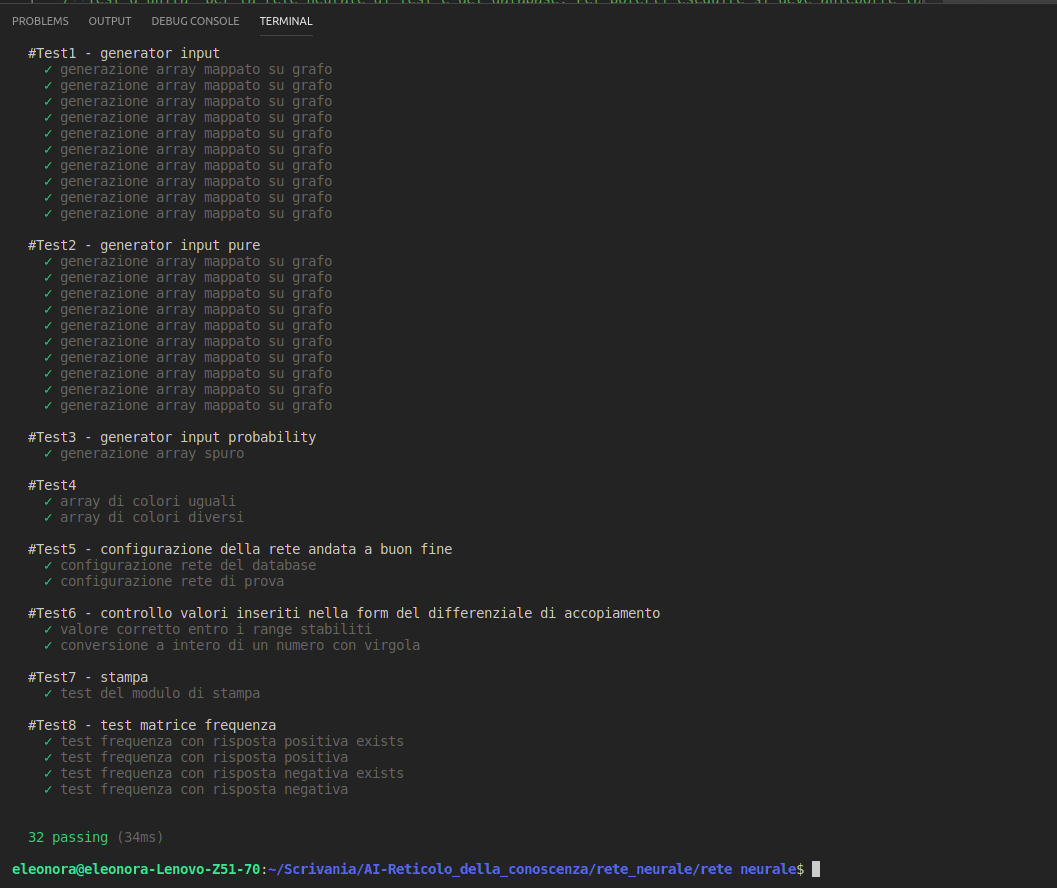
\includegraphics[width=0.80\linewidth]{./image/recap_test.png}
	\caption{Resoconto unit test con successo.}
	\label{Resoconto unit test con successo.}
\end{figure}
\noindent

\subsection{Sistema operativo e browser}
Il progetto \`e stato sviluppato su sistema operativo Linux e ripetutamente testato per tutta la durata dello stage sul sistema operativo Windows messo a disposizione in ufficio. L'applicativo della Rete neurale \`e sviluppato ad hov per browser Chrome; ma non ha mostrato alcuna problematica di adattabilit\`a n\`e su Firefox n\`e su Internet Explorer. Tuttavia sconsiglio l'utilizzo della Rete neurale in uso per i dati del database, in quanto la grande mole di dati rallenta eccessivamente l'operabilit\`a del browser. Il browser dove le attivit\`a della rete riscontrano una maggiore performance \`e Chorme.